% ============================================================================
\section{Classical ASR}
% ============================================================================

% Classical ASR: noisy channel, HMM--GMM, WFST decoders
\begin{frame}{Classical ASR: The Noisy Channel Model}
  \begin{itemize}
    \item \textbf{Search through space of all possible sentences.}
    \item \textbf{Pick the one that is most probable given the waveform.}
  \end{itemize}
  \begin{center}
    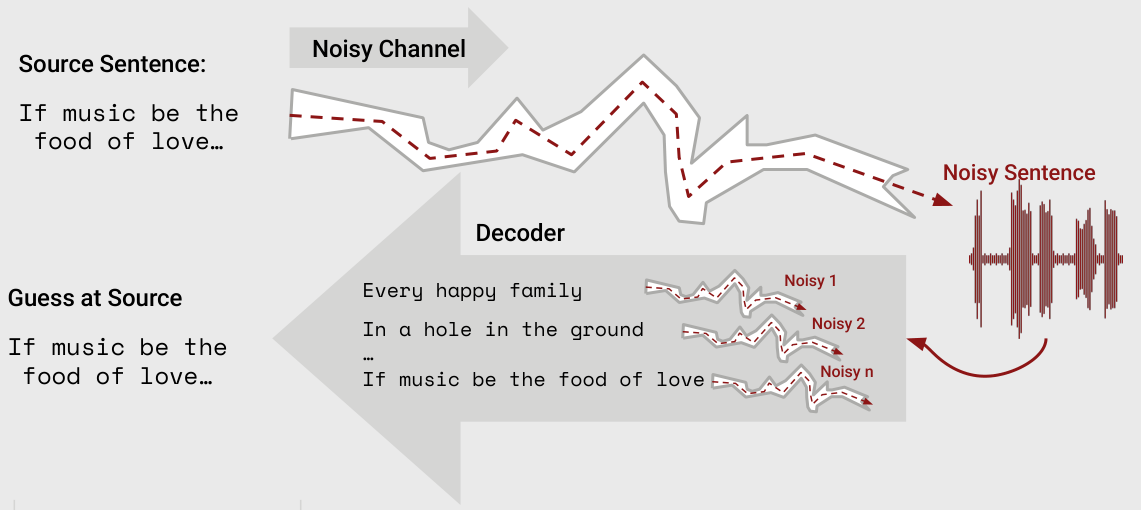
\includegraphics[width=\textwidth,height=0.92\textheight,keepaspectratio]{assets/New-Lecture-STT/cs224s_lec9_slide_05.png}
  \end{center}
\end{frame}

% --- Stanford CS224S lec9, slide 6 ---
\begin{frame}{The Noisy Channel Model}
  \begin{itemize}
    \item What is the most likely sentence out of all sentences in the language $L$ that generated some given
    \textbf{acoustic input} $O$?
    \item Treat acoustic input $O$ as sequence of individual observations:
    \begin{itemize}
      \item[] $O = o_1, o_2, \ldots, o_T$
    \end{itemize}
    \item Define a sentence as a sequence of words:
    \begin{itemize}
      \item[] $W = w_1, w_2, \ldots, w_n$
    \end{itemize}
  \end{itemize}
  \vfill
\end{frame}

% --- Stanford CS224S lec9, slide 7 ---
\begin{frame}{The Noisy Channel Model}
  \begin{itemize}
    \item \textbf{Probabilistic implication:} Pick the highest probability word sequence $W$:
      \begin{align*}
        \widehat{W} &= \arg\max\limits_{W \in L} P(W \mid O)
      \end{align*}
    \item \textbf{We can use Bayes' rule to rewrite this:}
      \begin{align*}
        \widehat{W} &= \arg\max\limits_{W \in L} \frac{P(O \mid W) P(W)}{P(O)}
      \end{align*}
    \item Since denominator is the same for each candidate sentence $W$, we can ignore it for the argmax:
      \begin{align*}
        \widehat{W} &= \arg\max\limits_{W \in L} P(O \mid W) P(W)
      \end{align*}
  \end{itemize}
  \vfill
\end{frame}

% --- Stanford CS224S lec9, slide 9 ---
\begin{frame}{The Noisy Channel Model}
  \centering
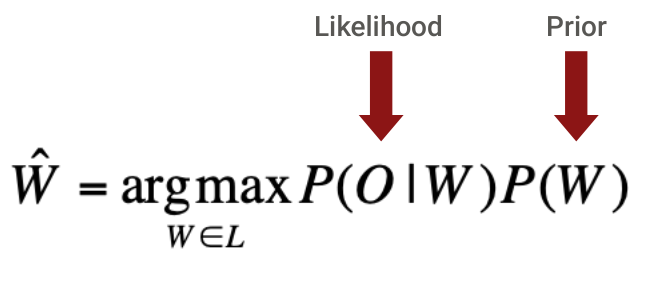
\includegraphics[width=\textwidth,height=0.92\textheight,keepaspectratio]{assets/New-Lecture-STT/cs224s_lec9_slide_09.png}
\end{frame}

% --- Stanford CS224S lec9, slide 11 ---
\begin{frame}{Word error rate (WER)}
\centering
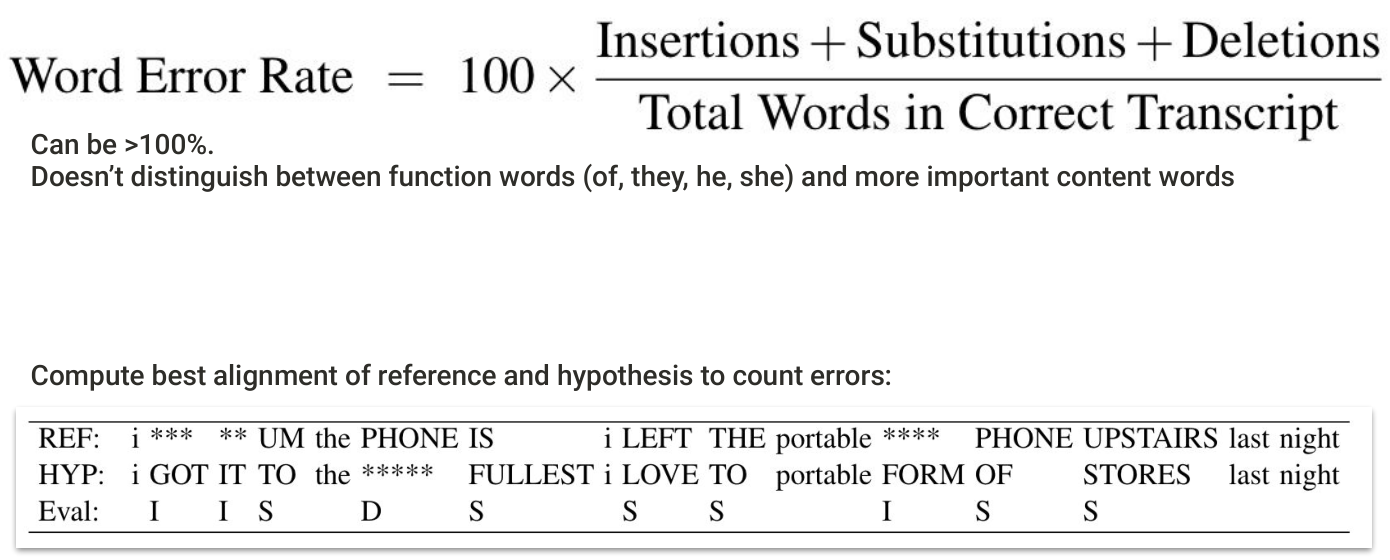
\includegraphics[width=\textwidth,height=0.92\textheight,keepaspectratio]{assets/New-Lecture-STT/cs224s_lec9_slide_11.png}
\end{frame}

\begin{frame}{Speech Recognition Architecture}
  \centering
  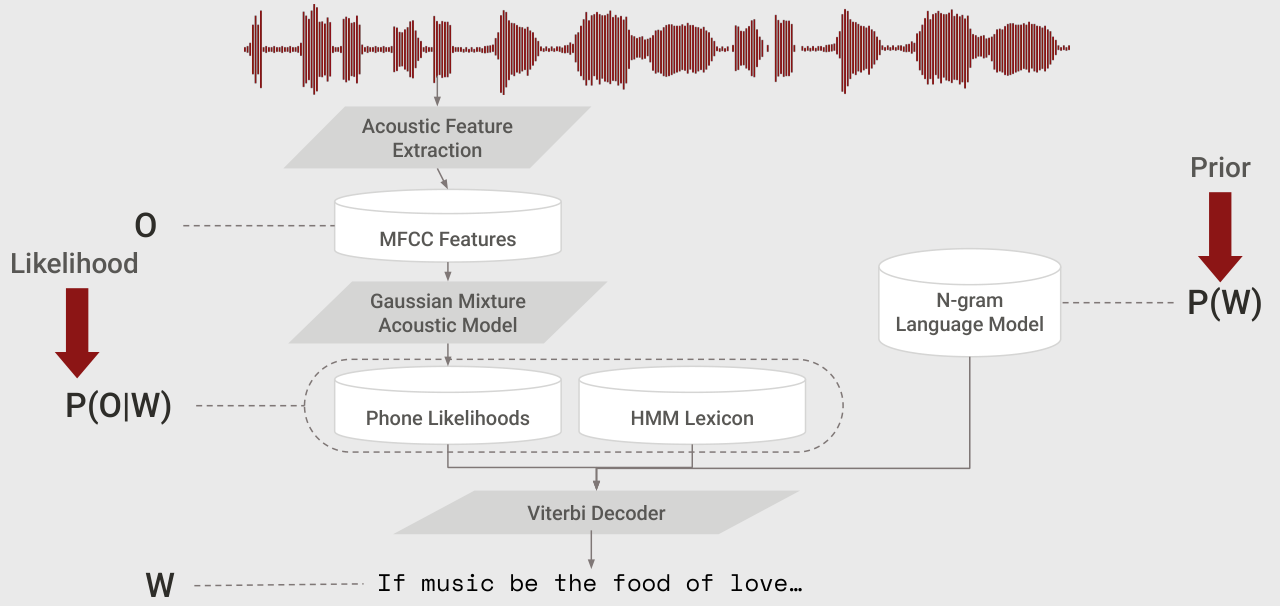
\includegraphics[width=\textwidth,height=0.92\textheight,keepaspectratio]{assets/New-Lecture-STT/cs224s_lec9_slide_13.png}
\end{frame}

% Classical ASR: HMM--GMM
% --- Stanford CS224S lec9, slide 16 ---
\begin{frame}{Classical ASR:HMM-GMM system}
  \centering
  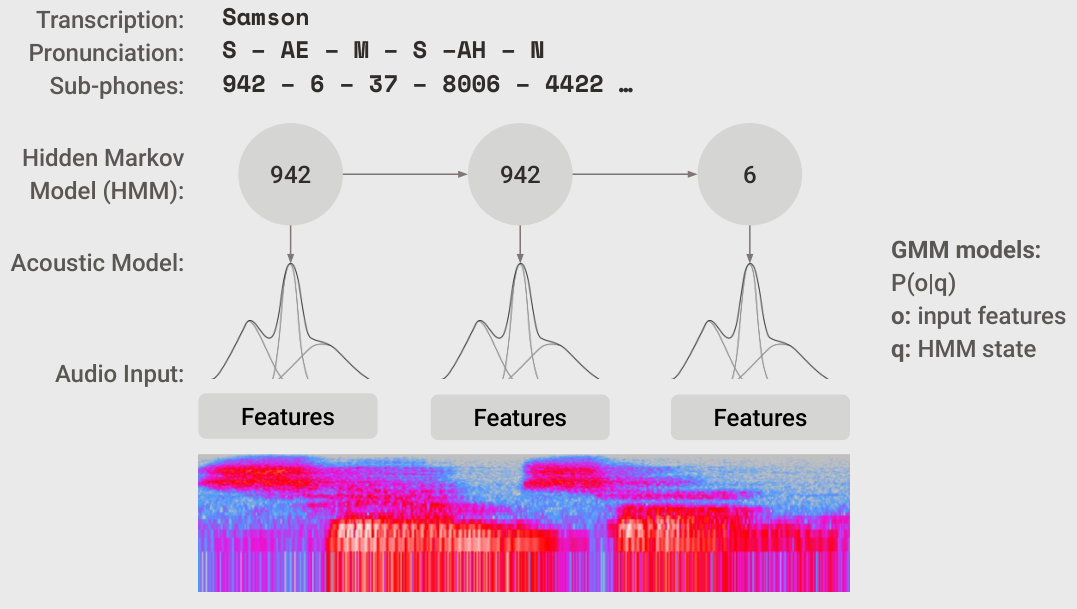
\includegraphics[width=\textwidth,height=0.92\textheight,keepaspectratio]{assets/New-Lecture-STT/cs224s_lec9_slide_16.png}
\end{frame}
